\problemname{Cave Escape}
For unknown reasons, you are exploring a cave and have accidentally awoken an angry bear.
The bear is bigger and faster than you, so your only chance is to outsmart it to get out.
The cave can be represented as a rectangular board consisting of walls and an exit.
You and the bear can move in the directions up, down, right, or left, but cannot walk through walls.

Each time you take a step, and have not reached the exit, the bear will respond by moving
up to $2$ steps in an attempt to get as close to you as possible. If you are ever on the same cell, you are lost.
Fortunately, the bear is not fully aware of walls, and therefore uses a dumb algorithm to move.

The first thing the bear does is move toward you in the horizontal direction. It does this until it runs out of steps,
hits a wall, or is in the same column as you. After that, it does the same thing in the vertical direction,
until it runs out of steps, hits a wall, or is in the same row as you. It is thus possible that the bear
moves $0$, $1$, or $2$ steps depending on where you are and where the walls are.

Given the layout of the cave, your task is to write a program that finds a sequence of moves that lets you escape the cave without being caught.

\begin{figure}[ht!]
\centering
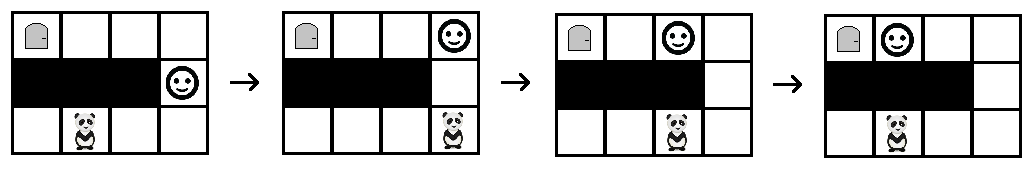
\includegraphics[width=\textwidth]{grottflykt.png}
\caption{An illustration of the first example}
\label{overflow}
\end{figure}

\section*{Input}
The first line contains two integers $w$ and $h$ ($ 3 \leq w*h \leq 64$), the width and height of the cave.

Then follow $h$ lines with $w$ characters each, a description of the cave. A wall is described with ``\#'', your starting position with ``S'',
the exit with ``U'', and the bear with ``B''. It is guaranteed that every test case has a solution. 

\section*{Output}
Output a line with a string consisting of the characters ``U'' for up, ``N'' for down, ``H'' for right, and ``V'' for left,
the steps you should take to escape the cave. An answer that walks into a wall at any point will not be accepted.
It is thus not possible to stand still for a turn by walking into a wall.

\noindent
\begin{tabular}{| l | l | p{12cm} |}
  \hline
  \textbf{Group} & \textbf{Points} & \textbf{Constraints} \\ \hline
  $1$    & $20$        & $h=1$ \\ \hline 
  $2$    & $30$        & $w*h \leq 25$ \\ \hline 
  $3$    & $50$        & No additional constraints. \\ \hline 
\end{tabular}
